\documentclass[tikz,border=5pt]{standalone}
\usepackage[T1]{fontenc}
\usepackage{lmodern}
\usepackage{xcolor}
\usetikzlibrary{arrows.meta,calc,fit,backgrounds}

\definecolor{ink}{HTML}{1C1917}
\definecolor{body}{HTML}{292524}
\definecolor{phys}{HTML}{1E5A8A}
\definecolor{physbg}{HTML}{F4F8FB}
\definecolor{time}{HTML}{6E568F}
\definecolor{timebg}{HTML}{F7F5FA}
\definecolor{woz}{HTML}{B8612E}
\definecolor{wozbg}{HTML}{FDF7F3}
\definecolor{part}{HTML}{2F7A58}
\definecolor{partbg}{HTML}{F3F8F5}
\definecolor{neutral}{HTML}{44403C}
\definecolor{serverbg}{HTML}{F3F2F1}
\definecolor{serverbd}{HTML}{D6D3D1}
\definecolor{dashc}{HTML}{57534E}

\newsavebox{\camerabox}
\savebox{\camerabox}{%
  
\begin{tikzpicture}[x=0.72ex,y=0.72ex,line cap=round,line join=round]
    \draw[neutral,line width=0.6pt,rounded corners=0.35pt] (0,0.15) rectangle (3.15,2.05);
    \draw[neutral,line width=0.6pt] (0.72,2.05) -- (1.02,2.62) -- (2.12,2.62) -- (2.42,2.05);
    \draw[neutral,line width=0.6pt] (1.58,1.08) circle (0.5);
    \fill[neutral] (1.58,1.08) circle (0.18);
  \end{tikzpicture}%
}
\newsavebox{\watchbox}
\savebox{\watchbox}{%
  
\begin{tikzpicture}[x=0.62ex,y=0.62ex,line cap=round,line join=round]
    \draw[phys,line width=0.55pt] (1.2,2.45) -- (1.42,2.95) -- (2.05,2.95) -- (2.28,2.45);
    \draw[phys,line width=0.55pt] (1.2,0.28) -- (1.42,-0.22) -- (2.05,-0.22) -- (2.28,0.28);
    \draw[phys,line width=0.65pt,rounded corners=0.45pt] (0.62,0.28) rectangle (2.85,2.45);
    \draw[phys,line width=0.55pt] (0.95,1.15) -- (1.25,1.45) -- (1.55,0.95) -- (1.9,1.35) -- (2.35,1.05);
  \end{tikzpicture}%
}

\begin{document}
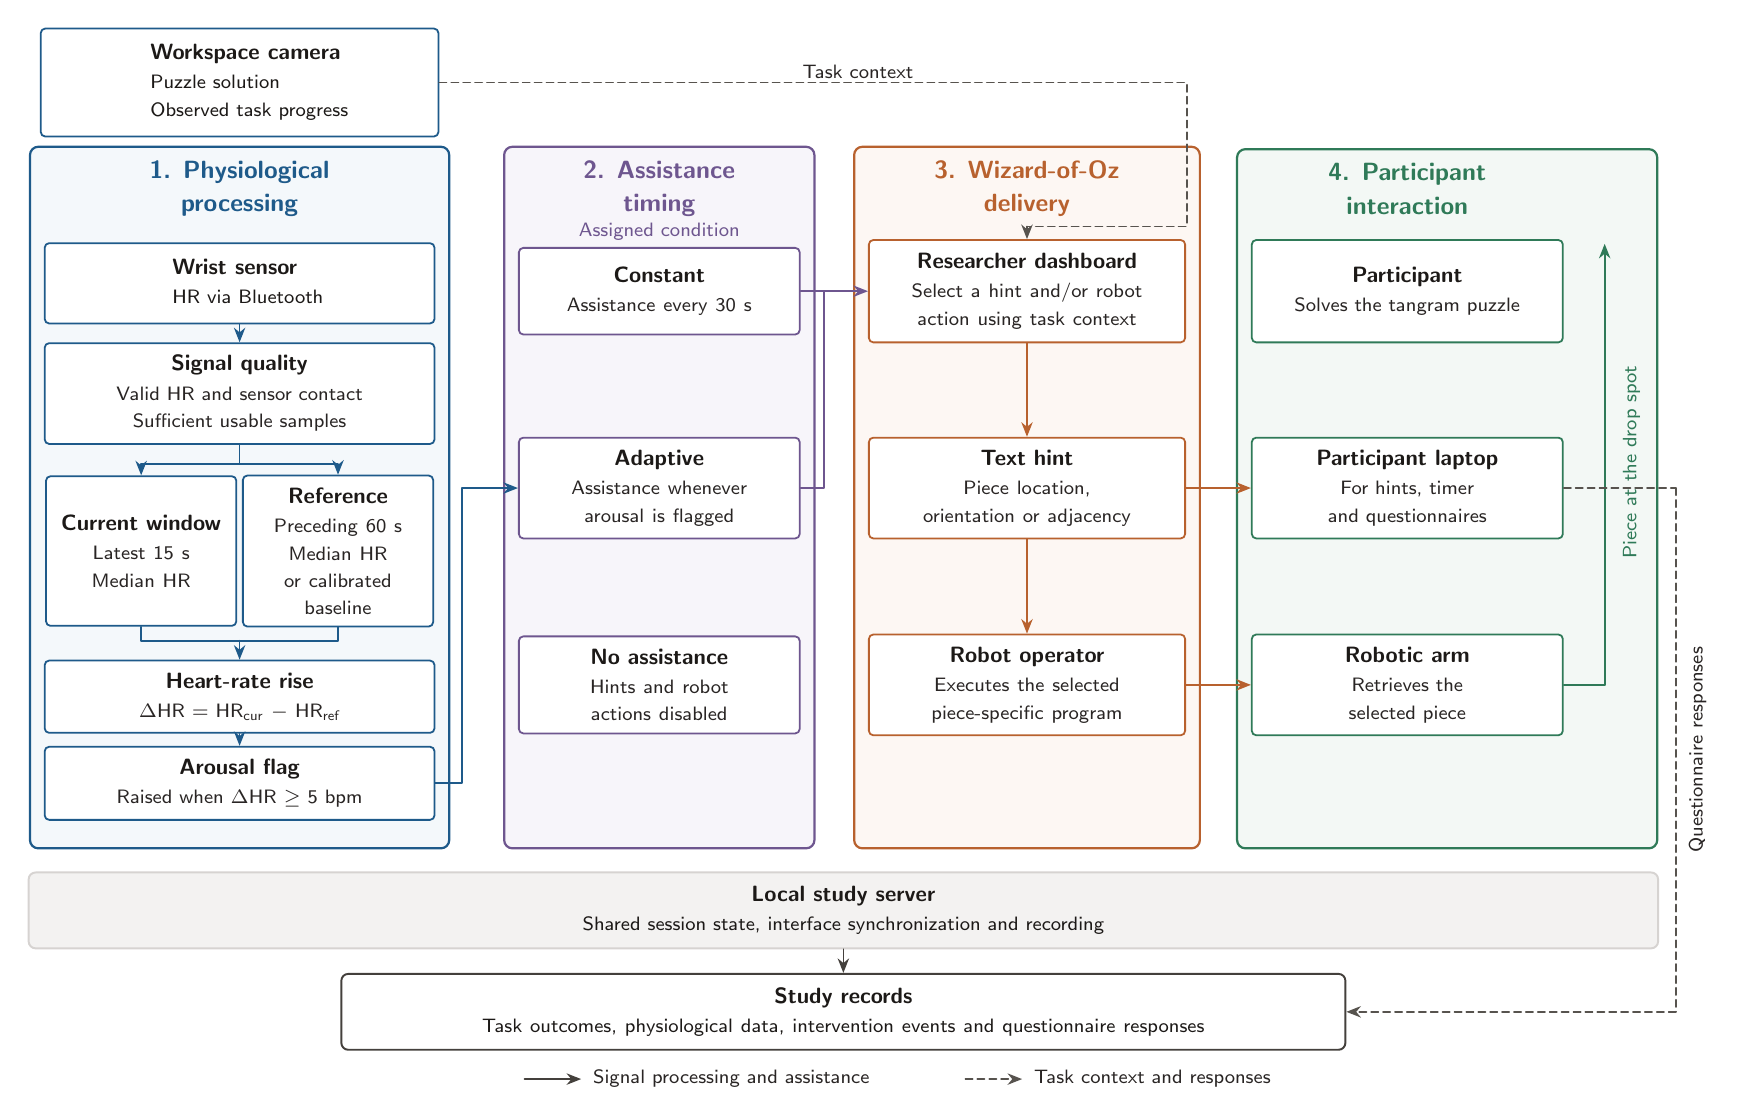
\begin{tikzpicture}[
  font=\sffamily,
  line cap=round,
  line join=round,
  arr/.style={-{Stealth[length=1.85mm,width=1.45mm]},line width=0.62pt},
  darr/.style={arr,dashed,dash pattern=on 2.6pt off 1.7pt,draw=dashc},
  rule/.style={line width=0.62pt},
  pbox/.style={
    draw,line width=0.65pt,rounded corners=1.6pt,fill=white,
    align=center,inner sep=4.5pt,font=\sffamily\footnotesize,text=ink
  },
  stage/.style={font=\sffamily\bfseries\small,align=center,inner sep=0pt},
  note/.style={font=\sffamily\scriptsize,text=body,inner sep=1pt}
]
\hyphenpenalty=10000
\exhyphenpenalty=10000

% Compact shared rows keep the cross-column arrows straight.
% Node spacing and panel padding reduced; labels and flow preserved.
\def\ax{2.72}
\def\bx{8.05}
\def\cx{12.72}
\def\dx{17.55}
\def\yTop{9.50}
\def\yMid{7.00}
\def\yLow{4.50}

% ---- Camera ----
\node[pbox,draw=phys,minimum width=5.05cm] (cam) at (\ax,12.15) {%
  \begin{tabular}{@{}c@{\hspace{7pt}}l@{}}
    \usebox{\camerabox} &
    \begin{tabular}{@{}l@{}}
      {\sffamily\bfseries\footnotesize Workspace camera}\\[1pt]
      {\sffamily\scriptsize Puzzle solution}\\[0.5pt]
      {\sffamily\scriptsize Observed task progress}
    \end{tabular}
  \end{tabular}%
};

\node[stage,text=phys] (t1) at (\ax,10.80) {1. Physiological\\[1pt]processing};
\node[stage,text=time] (t2) at (\bx,10.80) {2. Assistance\\[1pt]timing};
\node[stage,text=woz]  (t3) at (\cx,10.80) {3. Wizard-of-Oz\\[1pt]delivery};
\node[stage,text=part] (t4) at (\dx,10.80) {4. Participant\\[1pt]interaction};

% ---- 1. Physiological processing ----
\node[pbox,draw=phys,minimum width=4.95cm] (wrist) at (\ax,9.60) {%
  \begin{tabular}{@{}c@{\hspace{6pt}}l@{}}
    \usebox{\watchbox} &
    \begin{tabular}{@{}l@{}}
      {\sffamily\bfseries\footnotesize Wrist sensor}\\[1pt]
      {\sffamily\scriptsize HR via Bluetooth}
    \end{tabular}
  \end{tabular}%
};
\node[pbox,draw=phys,minimum width=4.95cm] (sq) at (\ax,8.20) {%
  {\bfseries Signal quality}\\[1pt]
  {\scriptsize\color{body} Valid HR and sensor contact}\\[0.5pt]
  {\scriptsize\color{body} Sufficient usable samples}%
};
\node[pbox,draw=phys,text width=2.10cm,minimum height=1.90cm] (cur) at (\ax-1.25,6.20) {%
  {\bfseries Current window}\\[1pt]
  {\scriptsize\color{body} Latest 15 s}\\[0.5pt]
  {\scriptsize\color{body} Median HR}%
};
\node[pbox,draw=phys,text width=2.10cm,minimum height=1.90cm] (ref) at (\ax+1.25,6.20) {%
  {\bfseries Reference}\\[1pt]
  {\scriptsize\color{body} Preceding 60 s}\\[0.5pt]
  {\scriptsize\color{body} Median HR}\\[0.5pt]
  {\scriptsize\color{body} or calibrated baseline}%
};
\node[pbox,draw=phys,minimum width=4.95cm] (hr) at (\ax,4.35) {%
  {\bfseries Heart-rate rise}\\[1pt]
  {\scriptsize\color{body} $\Delta$HR $=$ HR\textsubscript{cur} $-$ HR\textsubscript{ref}}%
};
\node[pbox,draw=phys,minimum width=4.95cm] (flag) at (\ax,3.25) {%
  {\bfseries Arousal flag}\\[1pt]
  {\scriptsize\color{body} Raised when $\Delta$HR $\geq$ 5 bpm}%
};

% ---- 2. Assistance timing ----
\node[note,text=time] (assigned) at (\bx,10.25) {Assigned condition};
\node[pbox,draw=time,text width=3.25cm,minimum height=1.10cm] (const) at (\bx,\yTop) {%
  {\bfseries Constant}\\[1pt]
  {\scriptsize\color{body} Assistance every 30 s}%
};
\node[pbox,draw=time,text width=3.25cm,minimum height=1.20cm] (adapt) at (\bx,\yMid) {%
  {\bfseries Adaptive}\\[1pt]
  {\scriptsize\color{body} Assistance whenever}\\[0.5pt]
  {\scriptsize\color{body} arousal is flagged}%
};
\node[pbox,draw=time,text width=3.25cm,minimum height=1.20cm] (none) at (\bx,\yLow) {%
  {\bfseries No assistance}\\[1pt]
  {\scriptsize\color{body} Hints and robot}\\[0.5pt]
  {\scriptsize\color{body} actions disabled}%
};

% ---- 3. Wizard-of-Oz delivery ----
\node[pbox,draw=woz,text width=3.7cm,minimum height=1.30cm] (dash) at (\cx,\yTop) {%
  {\bfseries Researcher dashboard}\\[1pt]
  {\scriptsize\color{body} Select a hint and/or robot}\\[0.5pt]
  {\scriptsize\color{body} action using task context}%
};
\node[pbox,draw=woz,text width=3.7cm,minimum height=1.20cm] (hint) at (\cx,\yMid) {%
  {\bfseries Text hint}\\[1pt]
  {\scriptsize\color{body} Piece location,}\\[0.5pt]
  {\scriptsize\color{body} orientation or adjacency}%
};
\node[pbox,draw=woz,text width=3.7cm,minimum height=1.20cm] (oper) at (\cx,\yLow) {%
  {\bfseries Robot operator}\\[1pt]
  {\scriptsize\color{body} Executes the selected}\\[0.5pt]
  {\scriptsize\color{body} piece-specific program}%
};

% ---- 4. Participant interaction ----
\node[pbox,draw=part,minimum width=3.95cm,minimum height=1.30cm] (person) at (\dx,\yTop) {%
  {\bfseries Participant}\\[1pt]
  {\scriptsize\color{body} Solves the tangram puzzle}%
};
\node[pbox,draw=part,minimum width=3.95cm,minimum height=1.20cm] (laptop) at (\dx,\yMid) {%
  {\bfseries Participant laptop}\\[1pt]
  {\scriptsize\color{body} For hints, timer}\\[0.5pt]
  {\scriptsize\color{body} and questionnaires}%
};
\node[pbox,draw=part,minimum width=3.95cm,minimum height=1.20cm] (arm) at (\dx,\yLow) {%
  {\bfseries Robotic arm}\\[1pt]
  {\scriptsize\color{body} Retrieves the}\\[0.5pt]
  {\scriptsize\color{body} selected piece}%
};

% Right-hand return sits inside the participant column.
\coordinate (rail) at ($(arm.east)+(0.52,0)$);
\node[note,text=part,rotate=90,anchor=center] (piecelab)
  at ($($(rail)!0.5!(rail |- person.north)$)+(0.34,0)$) {Piece at the drop spot};

\path (\ax,2.60) coordinate (b1)
      (\bx,2.60) coordinate (b2)
      (\cx,2.60) coordinate (b3)
      (\dx,2.60) coordinate (b4);

\begin{scope}[on background layer]
  \node[draw=phys,fill=physbg,line width=0.8pt,rounded corners=3pt,
        inner sep=5pt,fit=(t1)(wrist)(sq)(cur)(ref)(hr)(flag)(b1)] (F1) {};
  \node[draw=time,fill=timebg,line width=0.8pt,rounded corners=3pt,
        inner sep=5pt,fit=(t2)(assigned)(const)(adapt)(none)(b2)] (F2) {};
  \node[draw=woz,fill=wozbg,line width=0.8pt,rounded corners=3pt,
        inner sep=5pt,fit=(t3)(dash)(hint)(oper)(b3)] (F3) {};
  \node[draw=part,fill=partbg,line width=0.8pt,rounded corners=3pt,
        inner sep=5pt,fit=(t4)(person)(laptop)(arm)(piecelab)(b4)] (F4) {};
\end{scope}

% Physiological chain
\draw[arr,draw=phys] (wrist.south) -- (sq.north);
\coordinate (split) at ($(sq.south)+(0,-0.24)$);
\draw[rule,draw=phys] (sq.south) -- (split);
\draw[arr,draw=phys] (split) -| (cur.north);
\draw[arr,draw=phys] (split) -| (ref.north);
\coordinate (join) at ($(hr.north)+(0,0.24)$);
\draw[rule,draw=phys] (cur.south) |- (join);
\draw[rule,draw=phys] (ref.south) |- (join);
\draw[arr,draw=phys] (join) -- (hr.north);
\draw[arr,draw=phys] (hr.south) -- (flag.north);

% Arousal flag feeds Adaptive, up the gutter.
\draw[arr,draw=phys] (flag.east) -- ++(0.34,0) |- (adapt.west);

% Constant and Adaptive share one entrance into the dashboard.
\coordinate (gate) at ($(dash.west)+(-0.38,0)$);
\draw[rule,draw=time] (const.east) -- (gate);
\draw[rule,draw=time] (adapt.east) -- ++(0.30,0) |- (gate);
\draw[arr,draw=time] (gate) -- (dash.west);

% Wizard delivery
\draw[arr,draw=woz] (dash.south) -- (hint.north);
\draw[arr,draw=woz] (hint.south) -- (oper.north);
\draw[arr,draw=woz] (hint.east) -- (laptop.west);
\draw[arr,draw=woz] (oper.east) -- (arm.west);

% Piece returns upward inside the column.
\draw[rule,draw=part] (arm.east) -- (rail);
\draw[arr,draw=part] (rail) -- ($(rail |- person.north)+(0,-0.06)$);

% Task context: across the top, down the right of the delivery column, then into the dashboard.
\coordinate (ctx) at ($(F3.north east)+(-0.18,0)$);
\coordinate (ctxbend) at ($(dash.north)+(0,0.16)$);
\draw[rule,dashed,dash pattern=on 2.6pt off 1.7pt,draw=dashc]
  (cam.east) -- node[above,note,pos=0.56] {Task context} (cam.east -| ctx)
  -- (ctx |- ctxbend) -- (ctxbend);
\draw[darr] (ctxbend) -- (dash.north);

% Shared record
\path let \p1=($(F4.east)-(F1.west)$) in
  node[
    draw=serverbd,fill=serverbg,line width=0.7pt,rounded corners=2.5pt,
    minimum width=\x1,inner ysep=5pt,align=center,anchor=north,
    font=\sffamily\footnotesize,text=ink
  ] (server) at ($(F1.south)!0.5!(F4.south)+(0,-0.28)$) {%
    {\bfseries Local study server}\\[1pt]
    {\scriptsize Shared session state, interface synchronization and recording}%
  };

\node[
  draw=neutral,fill=white,line width=0.7pt,rounded corners=2.5pt,
  text width=12.4cm,align=center,inner sep=5pt,font=\sffamily\footnotesize,
  anchor=north,text=ink
] (records) at ($(server.south)+(0,-0.30)$) {%
  {\bfseries Study records}\\[1pt]
  {\scriptsize Task outcomes, physiological data, intervention events and questionnaire responses}%
};
\draw[arr,draw=neutral] (server.south) -- (records.north);

% Questionnaire responses leave the laptop and run down the outside.
\coordinate (qrail) at ($(F4.east)+(0.22,0)$);
\draw[rule,dashed,dash pattern=on 2.6pt off 1.7pt,draw=dashc]
  (laptop.east) -- (laptop.east -| qrail);
\draw[darr] (laptop.east -| qrail) -- (qrail |- records.east) -- (records.east);
\node[note,rotate=90,anchor=center]
  at ($($(laptop.east -| qrail)!0.5!(qrail |- records.east)$)+(0.28,0)$)
  {Questionnaire responses};

\coordinate (leg) at ($(records.south)+(0,-0.36)$);
\draw[arr,draw=neutral] ($(leg)+(-4.05,0)$) -- ++(0.72,0);
\node[note,anchor=west] at ($(leg)+(-3.22,0)$) {Signal processing and assistance};
\draw[darr] ($(leg)+(1.55,0)$) -- ++(0.72,0);
\node[note,anchor=west] at ($(leg)+(2.38,0)$) {Task context and responses};

\end{tikzpicture}
\end{document}
